\section{ФУНКЦИОНАЛЬНОЕ ПРОЕКТИРОВАНИЕ}
\label{sec:functional}

В данном разделе рассматривается проектирование системы на функциональном уровне, в
соответствии с полученной ранее структурной схемой. Для обеспечения модульности,
на данном уровне используются IP-ядра и стандартизированные протоколы обмена данными
между ними.

Разработка устройств на FPGA заметно облегчается механизмом IP-ядер (\en{Intellectual Property}) --- готовых
блоков для проектирования микросхем и прочих цифровых устройств. IP-ядра представляют собой
конфигурируемый блок цифрового устройства, описанный на HDL (\en{Hardware Description Language}).
Как правило, разработчик IP-ядра включает в него широкий перечень изменяемых параметров,
позволяя сторонним разработчикам переиспользовать ядро в своих целях, внося минимум необходимых
изменений вручную.

\subsection{Структура системы}
\label{sec:functional:structure}

Разрабатываемая система разделена на несколько блоков:

\begin{itemize}
  \item Video In to AXI4-Stream --- блок преобразования видеопотока в \en{AXI4-Stream};
  \item VDMA In --- Video DMA для входного видеопотока;
  \item Memory Interface Generator --- контроллер DDR-пямяти;
  \item VDMA Out --- Video DMA для выходного видеопотока;
  \item AXI CLKGEN --- генератор тактового сигнала для контроллера \en{HDMI};
  \item AXI HDMI TX --- блок управления контроллером \en{HDMI};
  \item AXI Camera I2C --- блок управления камерой посредством I2C;
  \item AXI HDMI I2C --- блок конфигурации контроллера \en{HDMI} посредством \en{I2C};
  \item AXI UART-Lite --- блок контроллера \en{UART};
  \item Microblaze --- soft-core микропроцессор для управления работой блоков;
  \item Microblaze Debug Module --- отладочный модуль для \en{Microblaze};
  \item Microblaze Local Memory --- локальная память \en{Microblaze};
  \item Processor System Reset --- контроллер сброса системы.
    % Докинуть сюда контроллер прерываний
\end{itemize}

Чертёж системы приведён ГУИР.400201.064 Э2.

\subsection{Video In to AXI4-Stream}
\label{sec:functional:video_in_to_axi4stream}
Большинство IP-ядер нацеленные на обработку видео используют протокол AXI4-Stream для
обмена данных. Передача видео между системами, обычно, сопровождается сигналами гашения и
синхросигналами для указания вертикальной и горизонтальной синхронизации, а также
валидности данных в видеопотоке. Интерфейс DVI (Digital Visual Interface) является
одним из представителей такого режима передачи. Ядро Video In to AXI4-Stream преобразует
входящий видеопоток и его управляющие и синхросигналы в протокол AXI4-Stream для
связи с другими блоками, поддерживающими данный протокол. На вход блоку поступает
видеопоток в параллельном виде, частота прорисовки одного пикселя и следующий набор
тайминговых сигналов:

\begin{itemize}
  \item Vsync, Hsync, Data Valid;
  \item Vblank, Hblank, Data Valid;
  \item Vsync, Hsync, Vblank, Hblank, Data Valid.
\end{itemize}

Для полноценной работы блока достаточно любого из этих трёх наборов сигналов. Выбор конкретного
множества существеннен при исползовании детектора Video Timing Controller.
Внутреннее устройство блока представлено на рисунке~\ref{fig:functional:vid_in_to_axi4stream:inner_structure}

\begin{center}
  \centering
  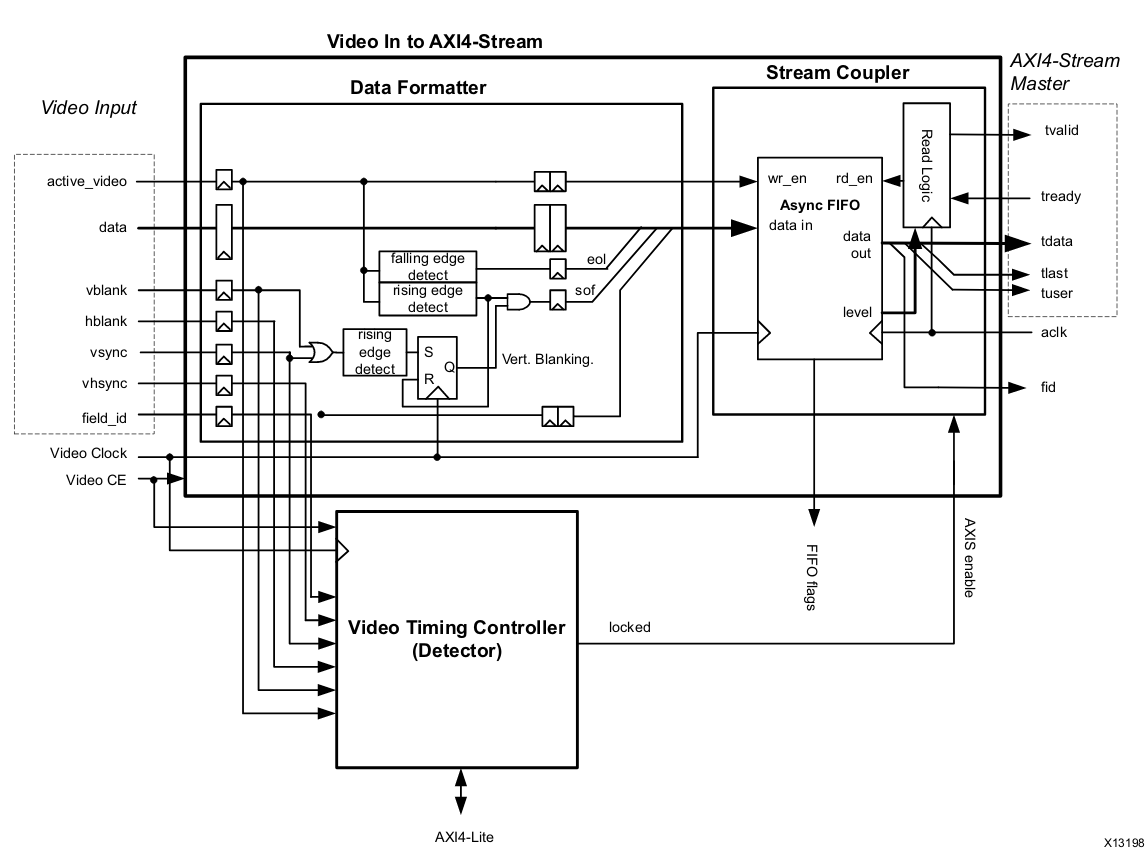
\includegraphics[scale=0.4]{vid_in_to_axi4stream.png}
  \captionof{figure}{ Структурная схема ядра Video In to AXI4-Stream }
  \label{fig:functional:vid_in_to_axi4stream:inner_structure}
\end{center}

Описание сигналов общего назначения:

\begin{itemize}
  \item ACLK --- тактовый сигнал шины AXI4-Stream, входной видеосигнал сэмплируется по фронту
    тактового импульса, выходной сигнал \en{AXI4-Stream} изменяется через некоторое время после фронта ACLK;
  \item ACLKE --- разрешение тактирования, активный высокий уровень. В случае подачи низкого уровня
    приостанавливает работу выходной шины, сохраняя внутреннее состояние блока. При переходе
    из низкого уровня в высокий входной видеопоток не сэмплируется, таким образом подавляя перезаписывание
    кадра в памяти блока.
  \item VCE (Video Clock Enable) --- разрешение работы внутренних регистов, отвечающих за работу с видео.
    Используется, когда видеосигнал подаётся с большей частотой, чем подразумевает стандарт синхронизации видео.
\end{itemize}

Описание видеосигналов приведено в таблице~\ref{table:functional:vid_in_to_axi4stream:video_signals}

\begin{table}[ht]
  \caption{Описание видеосигналов блока Video In to AXI4-Stream}
  \label{table:functional:vid_in_to_axi4stream:video_signals}
  \begin{tabular}{| >{\centering}m{0.18\textwidth}
                  | >{\centering}m{0.17\textwidth}
                  | >{\centering\arraybackslash}m{0.57\textwidth}|}
   \hline
    Обозначение сигнала & Разрядность & Краткое описание \\
    \hline
    ACTIVE & 1 & Валидность видеоданных. 1 --- активный видеопоток,
                        0 --- отсутствие видеоданных \\
    \hline
    DATA & 10 & Параллельный видеопоток \\
    \hline
    HBLNK & 1 & Строчный гасящий импульс, активный высокий уровень \\
    \hline
    HSYNC & 1 & Сигнал горизонтальной синхронизации, активный высокий уровень \\
    \hline
    VBLNK & 1 & Кадровый гасящий импульс, активный высокий уровень \\
    \hline
    VSYNC & 1 & Сигнал вертикальной синхронизации, активный высокий уровень \\
    \hline
  \end{tabular}
\end{table}

Описание сконвертированного видеопотока приведено в таблице~\ref{table:functional:vid_in_to_axi4stream:output_signals}

\begin{table}[ht]
  \caption{Описание выходных сигналов блока Video In to AXI4-Stream}
  \label{table:functional:vid_in_to_axi4stream:output_signals}
  \begin{tabular}{| >{\centering}m{0.18\textwidth}
                  | >{\centering}m{0.17\textwidth}
                  | >{\centering\arraybackslash}m{0.57\textwidth}|}
    \hline
    Обозначение сигнала & Разрядность & Краткое описание \\
    \hline
    TDAT & 32 & Видеоданные, соответствует AXI4-Stream TDATA \\
    \hline
    TVAL & 1 & Валидность видеоданных, соотвествует AXI4-Stream TVALID \\
    \hline
    TRDY & 1 & Готовность Slave-устройства принять данные, соотвествует AXI4-Stream TREADY \\
    \hline
    TLAST & 1 & Сигнал End of Line, соотвествует AXI4-Stream TLAST \\
    \hline
    TUSER & 1 & Начало нового кадра, соотвествует AXI4-Stream TREADY \\
    \hline
  \end{tabular}
\end{table}

По спецификации AXI4-Stream разрядность линий TDATA должна быть кратна 8-ю битам. % Вот тут хер пойми как правильно просклонять
Если входной видеопоток не кратен 8 битам, то данные должны быть дополнены нулями
начиная с старшего значащего бита. Таким же образом упакован выходной видеопоток.
На рисунке~\ref{fig:functional:vid_in_to_axi4stream:packed_output} показан
видеопоток с 12-ю битами на один канал формата RGB.

\begin{center}
  \centering
  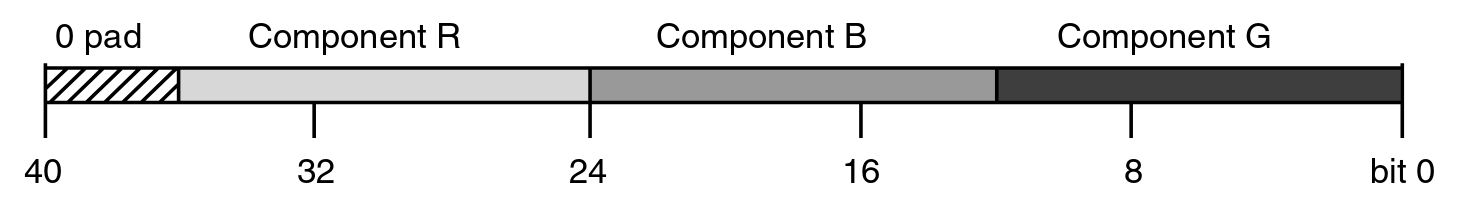
\includegraphics[scale=0.3]{vid_in_to_axi4stream_output.png}
  \captionof{figure}{ Упаковка выходного видеопотока в формате RGB }
  \label{fig:functional:vid_in_to_axi4stream:packed_output}
\end{center}

На входы блока подаётся видеопоток с CMOS-камеры. Для этого ядро конфиругируется в режим
\en{Image Sensor}, выбирается нужная разрядность (в данном случае 10 бит). Так как различные
матрицы выдают цветовые каналы в различном порядке, необходимо сконфигурировать порядок цветовых
каналов во входном видеопотоке.

При подключении камеры линии отрисовки пикселей, вертикальной и горизонтальной синхронизации,
валидности данных подключаются напрямую к контроллеру камеры, на линии VCE и ACLKE подаётся высокий уровень,
линия ACLK к общей линии тактирования системы. Для подачи выского или низкого уровня используется
специальный блок констант.

% Что нибудь ещё про камеру сказануть

\subsection{VDMA In}
\label{sec:functional:vdma_in}
Для обработки изменений в частоте кадров или изменения их размеров в приложениях
связанных с видеоконтентом используют кадровые буферы. Скоростной обмен между
таким буфером и системой обработки необходим: основные временные затраты
приходятся на передачу блоков данных из буфера и запись в него модифицированных частей кадра.

Ядро VDMA предоставляет возможность для высокоскоростного обмена между \en{AXI4-Stream} видеоинтерфейсом
и стандартным \en{AXI4}, разгружая управляющее устройство от активного контроля передачи.

Блок работает как стандартное устройство DMA, путём записи в регистры размера передаваемого блока данных,
начального адреса записи или чтения и количества циклов повторения операции. Оптимизация подобных
операций на микропроцессоре крайне затруднительна.

Блок VDMA оптимизирован для работы с непрерывным потоком данных, благодаря пакетному режиму передачи.
VDMA, в отличие от AXI DMA, имеет дополнительные линии для поддержки передачи видео без потери
сигналов развёртки и частоты отрисовки пикселей, что в дальнейшем можно использовать для смены частоты кадров.

%Добавить текст, чтобы всё съехало на новый лист
Внутреннее устройство блока представлено на рисунке~\ref{fig:functional:vdma_in:inner_structure}

\begin{center}
  \centering
  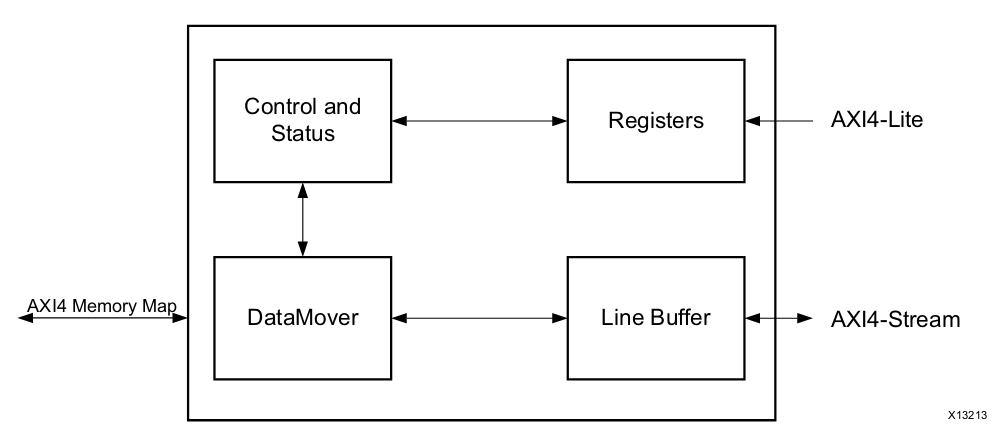
\includegraphics[scale=0.4]{vdma_structure.png}
  \captionof{figure}{ Структурная схема ядра VDMA }
  \label{fig:functional:vdma_in:inner_structure}
\end{center}

После программирования регистров по шине AXI4-Lite, блок управления и статуса генерирует список команд
для блока \en{DataMover}, чтобы инициировать команды чтения и записи интерфейса \en{AXI4 master}.
Асинхронный строковый буфер используется как временное хранилище пикселей с целью их последующей
записи на интерфейс \en{AXI4-Memory Map} или AXI4-Stream.

В случае записи VDMA прингимает кадры по slave интерфейсу AXI4-Stream и записиывает
их в память системы по master интерфейсу AXI4 master. В случае чтения ядро считывает
кадры по master интерфейсу AXI4 из системной памяти и перенаправляет их на master интерфейс
AXI4-Stream. Чтение и запись происходят независимо. Блок поддерживает возможность синхронизировать
входящие или исходящие кадры с внешним тактовым сигналом.

Основные возможности:
\begin{itemize}
  \item совместимость с протоколом AXI4 позволяет использовать модуль в любых приложениях, не разрабатывая
    собственный протокол высокоскоростной передачи данных;
  \item ядро поддеживает разрядность шины AXI4 в 32, 64, 128, 256, 512 и 1024 бита;
  \item ядро поддеживает разрядность шины AXI4-Stream по множителям 8 до 1024 бит;
  \item встроенные 32 кадровых буфера для 32-битного адресного пространства;
  \item опционально используется контроллер автоматического выравниваения обращений к памяти,
    транслируя обращение к произвольному адресу в выровненное. Поддерживается вплоть до 64-битной
    шины \en{AXI4-Stream};
  \item каждый канал VDMA может быть синхронизирован с другим при помощи \en{Genclock}, не позволяя
    при этом обоим каналам обращаться к одному и тому же кадровому буферу;
  \item поддержка асинхронных синхросигналов для различных типов AXI интерфейсов;
  \item блок способен динамически изменять частоту тактирования AXI4-Stream интерфейса,
    что позволяет передавать кадры с частотой и разрешением, отличным от исходных;
  \item поддержка различных механизмов синхронизации кадров, используя пользовательские линии
    шин AXI4.
\end{itemize}

Описание входных сигналов общего назначения приведено в таблице~\ref{table:functional:vmda_in:common_signals}

\begin{table}[ht]
  \caption{Описание входных сигналов общего назначения блока VDMA}
  \label{table:functional:vmda_in:common_signals}
  \begin{tabular}{| >{\centering}m{0.18\textwidth}
                  | >{\centering}m{0.17\textwidth}
                  | >{\centering\arraybackslash}m{0.57\textwidth}|}
   \hline
    Обозначение сигнала & Разрядность & Краткое описание \\
    \hline
    SC & 1 & тактовый сигнал AXI4-Lite \\
    \hline
    S2MC & 1 & тактовый сигнал AXI4-Stream to Memory Map \\
    \hline
    SS2MC & 1 & тактовый сигнал slave AXI4-Stream to Memory Map \\
    \hline
    ARST & 1 & сигнал сброса AXI4-Lite \\
    \hline
    ACLK & 1 & тактовый сигнал шины AXI4-Lite \\
    \hline
  \end{tabular}
\end{table}

Рассмотрим сигналы, используемые во входном VDMA при считывании кадров с преобразователя и последующей их передаче
в оперативную память. Для этого применяется 3 AXI интерфейса: AXI4-Lite для конфигурации ядра,
slave интерфейс AXI4-Stream to Memory Map для считывания входящего видеопотока и master интерфейc AXI4
для записи потока в оперативную память.